% TODO:
%   o Rose mentions centrality; important for us?

\section{Introduction}

%% Points to make:
%% - Why forum important
%%     o For humanities
%%     o For helping each other
%% - Not all participate
%%     o why?
%%     o Observing actions every week to predict dropout.
%%       Maybe had forum actions?:
%%       Balakrishnan Girish. Predicting Student Retention in Massive
%%       Open Online Courses using Hidden MarkovModels. EECS Department,
%%       University of California, Berkeley, May, 2013.   

%% - Residential is different from MOOCs:
%%     o Incentives: more at stake after drop-out
%%     o Problem of forum cliques falling apart from
%%       course attrition goes away.
%%     o No late-comers that stay at the periphery
%%         (Rose:Turn-off)
%%     o Possible prior acquaintance
%%     o Smaller
%% - We have evidence that encouragement tricky
%%     o Grade: reduces intrinsic motivation.
%%     o Appeal to personal growth: negative
%%     o Appeal to community ?
%%     o These interventions were at the start, when
%%         urgency not there yet.
%% - Now: many courses available: reruns and varied
%%     o We can see dynamics of forum participation
%%       over time through a course. For top and
%%       average students.
%%     o When do prolific students tend to get engaged?
%%     o At any point in time, can we see a
%%       trajectory of prolific and median students?

%% - Analyzed the graph, snapshots over time. Are there
%%   inflection points?

%%     o Cite
%%       [14] Borgatti, Stephen P. Centrality and network flow. Social
%%       networks 27.1 (2005): 55-71. Rose uses their interpretation of
%%       what the social graphs mean 
%%     o Identify places where encouragement could be given.
%%       Inflection points?

%%     o We don't discuss the *form* of encouragement, though
%%       the messaging is important:

%%       * These say that emotional support is important:

%%         [13] Wang, Yi-Chia, Robert Kraut, and John M. Levine. To stay
%%         or leave?: the relationship of emotionaland informational support
%%         to commitment in online health support groups. Proceedings of the
%%         ACM 2012conference on Computer Supported Cooperative Work. ACM,
%%         2012.       
%%       * Could appeal to personal gain for forum participation,
%%       * Could appeal to community gain for forum participation,
%%       * Could just state facts.

\section{Introduction}


\section{From Posts to Connection Graph}

Social networks are most simply modeled by considering each
participant as a node, and interactions initiated by participants as
out-directed links. In this case all nodes are of one type, and links
are unidirectional. Multiple interaction initiations by one person are
captured by weighting the corresponding outgoing links. Many graph
analysis tools operate on models of this type, and this is the
approach we chose.

However, other strategies exist to cover different goals. For example,
\cite{Anwar2013} additionally consider linkages between forum post
topics to include communication content in the model. When networks
operate on particular platforms, such as underground forums, which
include private `buddy' connections, such facilities may need to be
modeled \cite{Moto2011}.

For the purpose of identifying candidate time points for encouraging
online conversation participation our chosen model suffices. We are
not in this work considering additional measures, such as content
quality, for which a richer model would be required.

Many measures are used to quantify various aspects of social graphs
\cite{***}. Not all are meaningful in the context of education-related
forum interactions. We focus here on two measures: {\em out-degree},
and {\em page rank}. Figure~\ref{fig:graphExpl} illustrates.

\begin{figure}[htp]
       \centering
       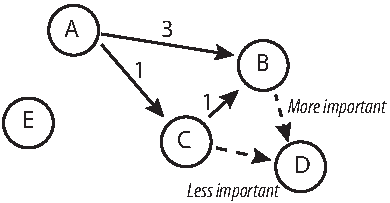
\includegraphics[width=1.0\textwidth]{Figs/forumNetworkExample.pdf}
       \caption{\textnormal{Example social graph induced by forum posts.}}
       \label{fig:graphExpl}
\end{figure}

Nodes $A$, $B$, $C$, $D$, and $E$ represent students. The link from
$A$ to $B$ is marked with the number $3$, because $A$ commented three
times on one of more of $B$'s posts. The number of outgoing links is
the node's {\em out-degree}. For example, the {\em out-degree} of $A$
is $4$.

The number of incoming links is called the node's {\em
  in-degree}. Node $C$'s in-degree is $1$. Node $E$ has no links
entering or exiting. The respective student has not participated in
the forum.

Analogous to Web pages, each node can be assigned a {\em page
  rank}. The intuition in this context is that student $S_1$'s
presence in the forum is more `important' than student $S_2$'s if the
node representing $S_1$ has higher page rank than the node that
represents $S_2$. In our context the intuition behind page rank is
that a node $N$ is more important (has higher page rank) the more
other important nodes comment on $N$'s posts. Imagine a scenario
in which student $S_1$ posts an interesting question, to which many
students comment with their opinion, creating a long thread. The node
representing $S_1$ would experience an increase of its page rank with
every incoming comment. Node $B$ in Figure~\ref{graphExpl} is an
example for this situation. Its in-degree is $4$. If $B$ were to
comment on one of $D$'s posts, then $D$'s page rank would increase
more than if the low-page-rank node $C$ commented on $D$.

In terms of evaluating a student's participation in the forum, a high
page rank, and high out-degree are positive. Low values are less
positive. We chose these two values because of their relatively
straight-forward meanings when applied to forum posts, and for their
relevance to our goal of identifying potential intervention times.

Some of the fifteen other measures we computed, such as {\em
  betweenness} are meaningful for forum scenarios as well, but their
usefulness depends on one's analysis goals. For example,
\cite{yang2013} include several of those measures for the purpose of
prediction analysis. For evaluation contribution quality the contents
of posts would need to be considered: students who persistently post
irrelevant contents contribute less positively to the forum than
constructively participating students. However, for our purposes the
two measures of page rank and out-degree provide strong enough
signals.

\section{Analysis Procedure}

We computed our chosen social graph measures for 39 offerings of seven
residential courses, and for one MOOC. Table~\ref{tab:courseSummary}
summarizes these data sources. We recomputed the measures for every
week throughout the quarter of each offering. In order to establish
values against which to compare each student's measures during those
weekly checkpoints we each time computed the two measures for ({\em
  i}) the average of the ten students who overall contributed the
maximum number of posts, and ({\em ii}) for the median number of
contributions at each checkpoint.

\begin{table*}[]
\centering
\caption{Summary of Examined Courses}
\label{tab:courseSummary}
\begin{tabular}{|l|c|c|l|l|}
\hline
\multicolumn{1}{|c|}{\textbf{Topic}}                            & \textbf{Offerings} & \textbf{Num-Students} & \multicolumn{1}{c|}{\textbf{Num-Active-Students}} & \multicolumn{1}{c|}{\textbf{Encouragement}} \\ \hline
\begin{tabular}[c]{@{}l@{}}Computational\\ Biology\end{tabular} & 5                  & 120                   &                                                   &                                             \\ \hline
Artificial Intelligence                                         & 7                  & 340                   &                                                   &                                             \\ \hline
Machine Learning                                                & 7                  & 640                   &                                                   &                                             \\ \hline
Computer Vision                                                 & 5                  & 144                   &                                                   &                                             \\ \hline
Decision Analysis                                               & 4                  & 232                   &                                                   &                                             \\ \hline
Audio Signal Processing                                         & 6                  & 21                    &                                                   &                                             \\ \hline
Political Methodology                                           & 5                  & 23                    &                                                   &                                             \\ \hline
\end{tabular}
\end{table*}


\begin{figure}[htp]
       \centering
       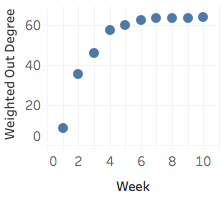
\includegraphics{Figs/women_health_summer2015_top10.png}
       \caption{\textnormal{A MOOC forum post comparison: Women's
           Global Health.}}
       \label{fig:womenHealth}
\end{figure}


\section{Conclusion and Future Work}

Here is an example chart of the correct size.
\begin{figure}[htp]
       \centering
       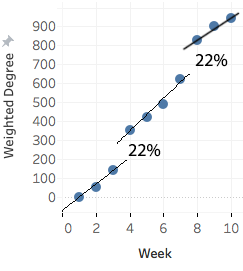
\includegraphics{Figs/exampleChart1.png}
       \caption{\textnormal{Wrong numbers, just an example. See ~/tmp/forumPromptsTableauChartsSample.twb}}
       \label{fig:exampleChart}
\end{figure}


\begin{itemize}
\item Consider student post content quality
\item Consider consistency: contribute throughout course
\item Consider influence on others
\item Draw instructor attention to dense topic clusters, which might
  indicate confusion, or student excitement to harness.
\end{itemize}
